\documentclass[UTF8,a4paper,12pt]{ctexart}
\usepackage[left=2.4cm,right=2.4cm,top=2.6cm,bottom=2.6cm]{geometry}
\usepackage{amsmath,booktabs,array,graphicx}
\usepackage{caption}

\title{\textbf{Patch Test 加入 $K_g$ 後的簡要匯報}}
\author{}
\date{\today}

\begin{document}
\maketitle

\section*{1. 使用了什麼代碼}

本次測試使用的主程式為：
\begin{itemize}
  \item \texttt{src/patch\_test.jl}
\end{itemize}

其中主要使用到的 operator 為：
\begin{itemize}
  \item \texttt{int kappa-kappa}：彎曲剛度
  \item \texttt{int w-w}：撓度相關剛度
  \item \texttt{int phi-phi}：轉角剛度
  \item \texttt{int phi-w}：轉角與撓度耦合項
  \item \texttt{int w-w-G}：幾何剛度項 $K_g$
\end{itemize}

\section*{2. 更改或加入了什麼代碼}

原本系統矩陣只組成材料剛度矩陣：
\begin{equation}
K=
\begin{bmatrix}
K_{\phi\phi} & K_{\phi w}\\
K_{w\phi} & K_{ww}
\end{bmatrix}.
\end{equation}

這次新增的部分是幾何剛度矩陣：
\begin{equation}
K_g=
\begin{bmatrix}
0 & 0\\
0 & G_{ww}
\end{bmatrix},
\end{equation}

\begin{center}
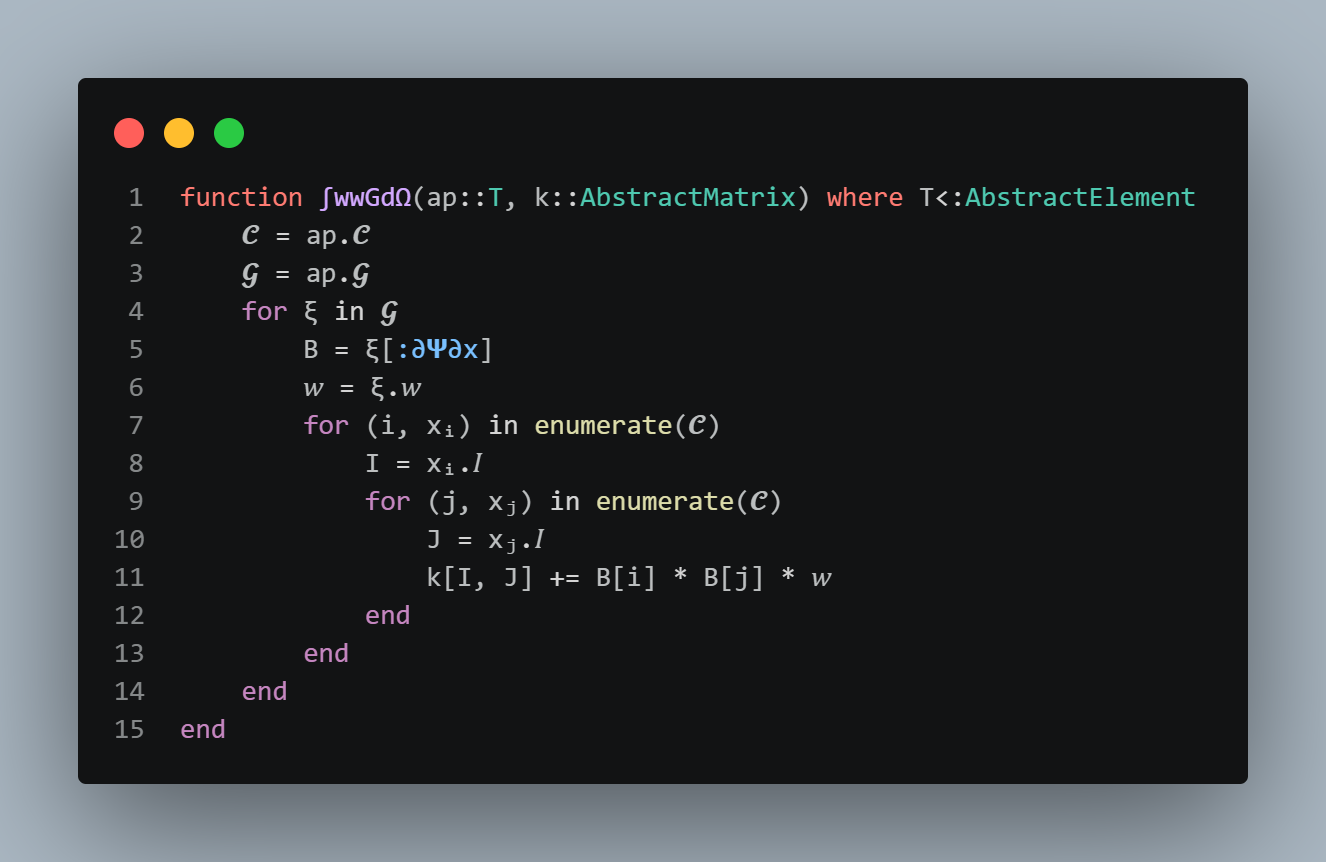
\includegraphics[width=0.88\linewidth]{code2.png}
\captionof{figure}{$K_g$ 公式程式碼（code2.png）}
\end{center}

對應程式是：
\begin{itemize}
  \item 將求解式由
  \begin{equation*}
  Kd=f
  \end{equation*}
  改成
  \begin{equation*}
  (K-K_g)d=f
  \end{equation*}
\end{itemize}

\begin{center}
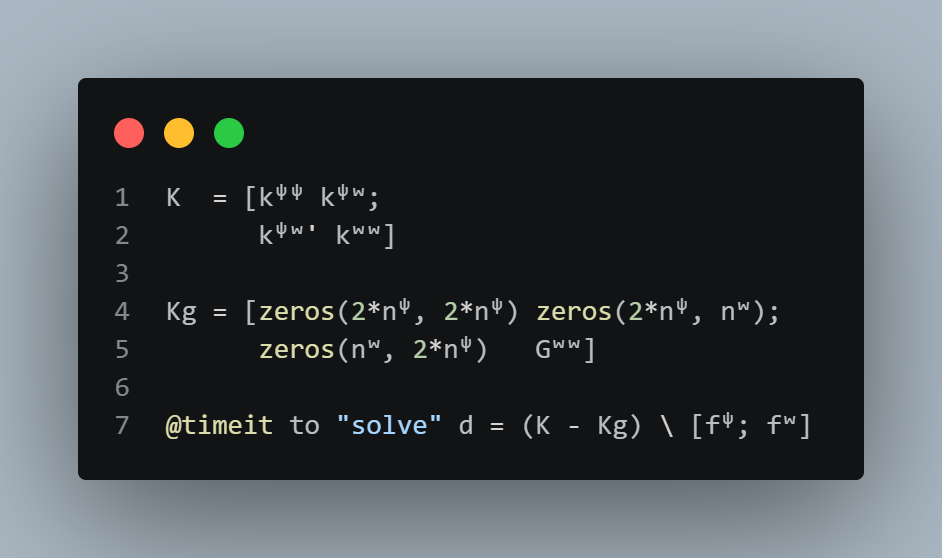
\includegraphics[width=0.88\linewidth]{code1.png}
\captionof{figure}{矩陣計算程式碼（code1.png）}
\end{center}

\section*{3. 結果對比如何}

\begin{table}[h]
\centering
\caption{加入與未加入 $K_g$ 的誤差比較}
\begin{tabular}{>{\raggedright\arraybackslash}p{3.0cm}cc}
\toprule
案例 & $L_2$ error of $w$ & $L_2$ error of $\phi$ \\
\midrule
有 $K_g$ & $2.6340759263762195\times 10^{-8}$ & $7.910863209601133\times 10^{-6}$ \\
沒有 $K_g$ & $7.030564851229914\times 10^{-7}$ & $8.910095366951204\times 10^{-6}$ \\
\bottomrule
\end{tabular}
\end{table}

從結果可以直接整理成：
\begin{itemize}
  \item 加入 $K_g$ 後，$w$ 的誤差由 $7.03\times 10^{-7}$ 降到 $2.63\times 10^{-8}$，明顯變小。
  \item 加入 $K_g$ 後，$\phi$ 的誤差由 $8.91\times 10^{-6}$ 降到 $7.91\times 10^{-6}$，也有小幅改善。
  \item 因此這次加入 $K_g$ 之後，對 patch test 的結果整體是正向的，尤其對撓度 $w$ 的改善最明顯。
\end{itemize}

\end{document}
